\section{Finding an obvious curve}

We build a grammar from a single curve, using a hand-picked
decomposition.

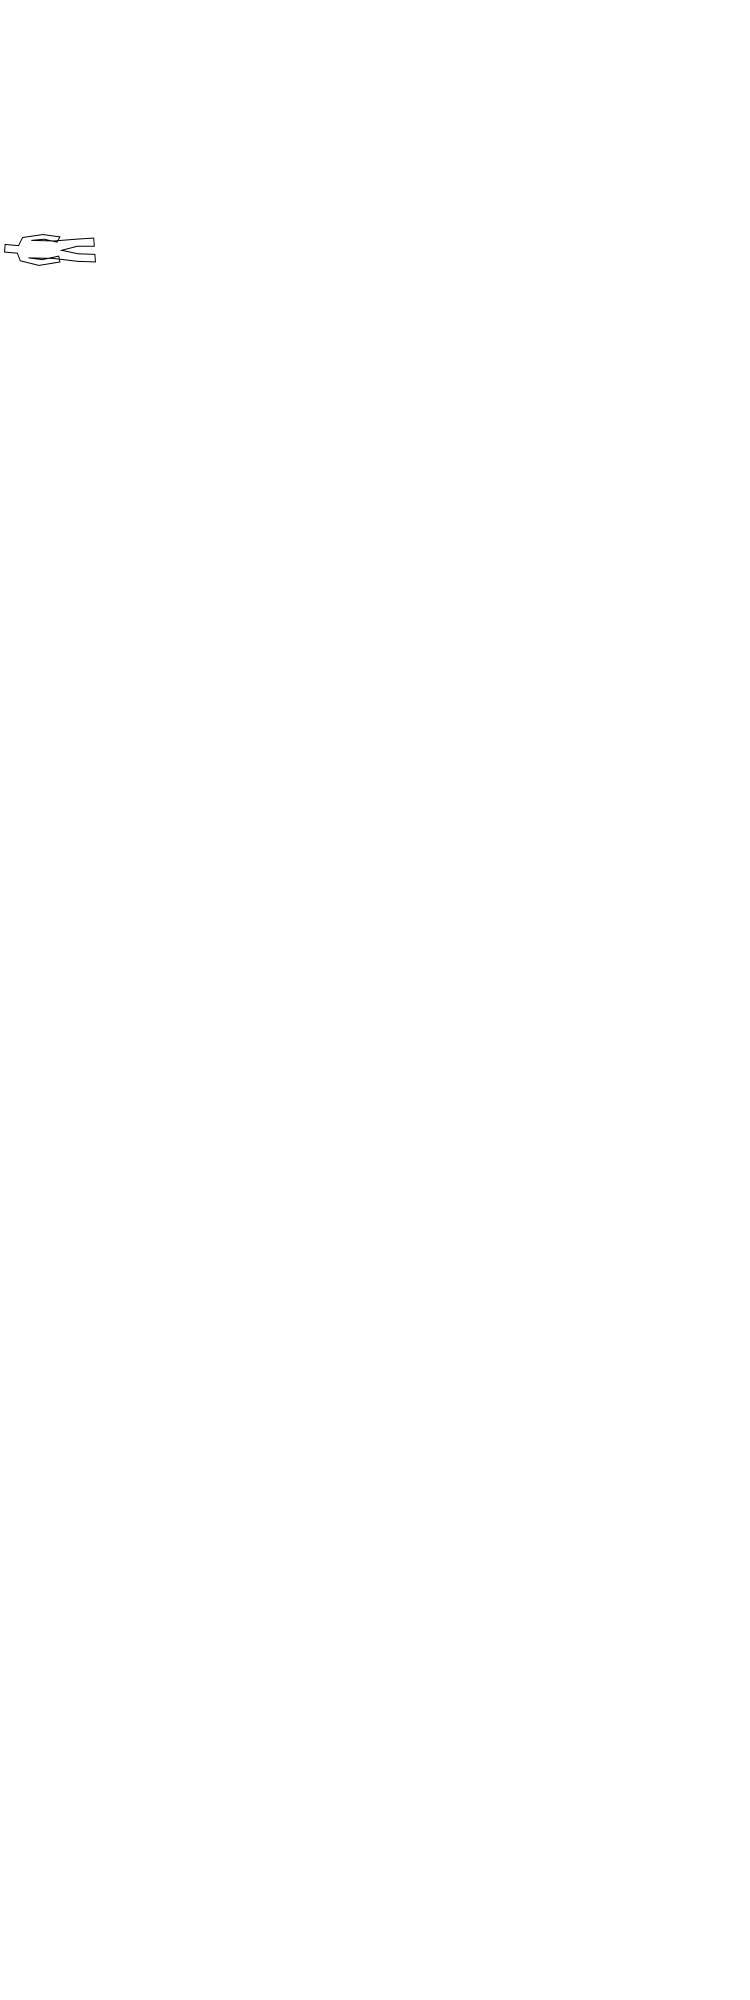
\includegraphics[width=4in]{experiments/4.images/standard_cky/output.d/examples.png}

We then pick some other curves which we wish to parse:

\includegraphics[width=4in]{experiments/4.images/standard_cky/output.d/targets.png}

We build a simple network on a 16x16 grid. We give curve segments a
data cost of 1.0, and short non-curve segments a data cost of 100.0.
On the left are the points of the network, with the curve segments
shown. On the right is the parse found.

\begin{center}
\begin{tabular}{ll}
\hline
 \includegraphics[width=10em]{experiments/4.images/standard_cky/output.d/network.0000.eps}  &
 \includegraphics[width=10em]{experiments/4.images/standard_cky/output.d/cky.im0000.final.png}  \\
\hline
 \includegraphics[width=10em]{experiments/4.images/standard_cky/output.d/network.0010.eps}  &
 \includegraphics[width=10em]{experiments/4.images/standard_cky/output.d/cky.im0010.final.png}  \\
\hline
\end{tabular}
\end{center}

